\documentclass[twocolumn]{article}
\usepackage{graphicx}
\usepackage{lipsum} % For generating dummy text
\usepackage{multicol}
\usepackage{subcaption}

\begin{document}

\title{Your Title}
\author{Your Name}
\date{\today}
\maketitle

\begin{abstract}
Your abstract goes here.
\end{abstract}

\begin{multicols}{2}
    \noindent
    \textbf{Theoretical Time Complexities}

    To provide a theoretical context for our empirical findings, we include graphs representing the time complexities of \(O(n^2)\) and \(O(n \log n)\) in Figure \ref{fig:theoretical_complexities}.

    The theoretical complexities serve as a reference point, confirming that the observed performance aligns with the expected behaviors of Selection Sort and TimSort.

    \begin{figure*}[h]
        \centering
        \begin{subfigure}{0.4\textwidth}
            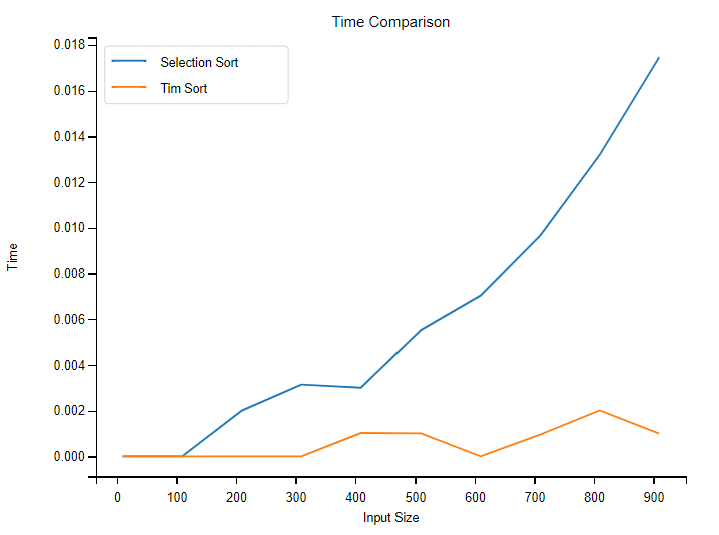
\includegraphics[width=\linewidth]{Images/900_time_comp.png}
            \caption{For data size: 900}
            \label{d900}
        \end{subfigure}
        \hfill
        \begin{subfigure}{0.4\textwidth}
            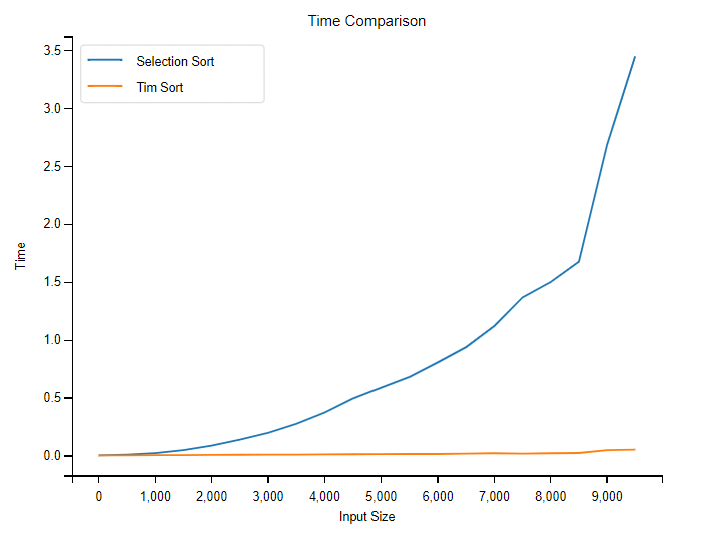
\includegraphics[width=\linewidth]{Images/9k_time_comp.png}
            \caption{For data size: 9000}
            \label{d9k}
        \end{subfigure}
        \hfill
        \begin{subfigure}{0.4\textwidth}
            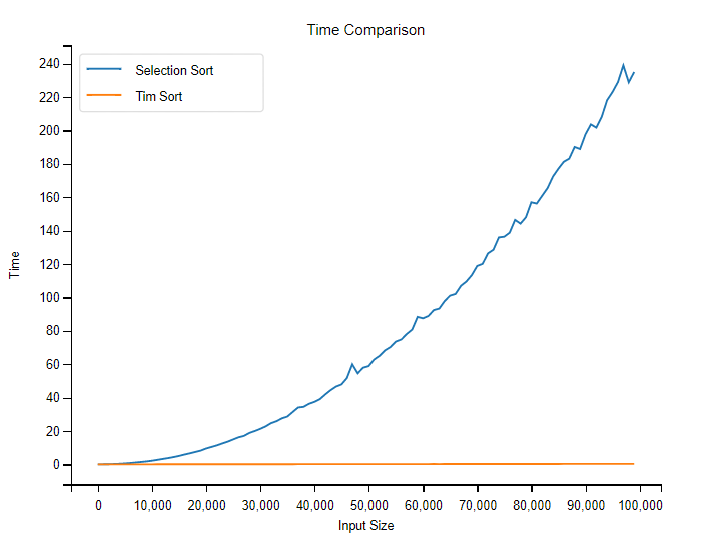
\includegraphics[width=\linewidth]{Images/100k_time_comp.png}
            \caption{For data size: 100,000}
            \label{d100k}
        \end{subfigure}
        \caption{Time Comparison between Selection and TimSort}
        \label{fig:theoretical_complexities}
    \end{figure*}

    In summary, our empirical results and theoretical considerations collectively suggest that TimSort is a more efficient sorting algorithm compared to Selection Sort, especially in scenarios with larger datasets.
\end{multicols}

\end{document}
